\documentclass[crop,tikz]{standalone}% 'crop' is the default for v1.0, before it was 'preview'
%\usetikzlibrary{...}% tikz package already loaded by 'tikz' option
\usepackage{color}
\newcommand{\gv}[1]{\ensuremath{\mbox{\boldmath$ #1 $}}} 
\renewcommand{\v}[1]{\ensuremath{\mathbf{#1}}}
\newcommand{\name}[1]{_{\text{#1}}}
\usepackage{siunitx}
\usetikzlibrary{shapes,arrows,shadings,backgrounds,calc}
\definecolor{brown}{rgb}{0.59, 0.29, 0.0}
\begin{document}
    \begin{tikzpicture}
    %% \node(a)at(2,0){
    %%   \begin{tikzpicture}[scale=1, every node/.style={scale=1}]
    %%     \node[label={[yshift=-0.2cm] \scriptsize Initial configuration}](a) at(0,0){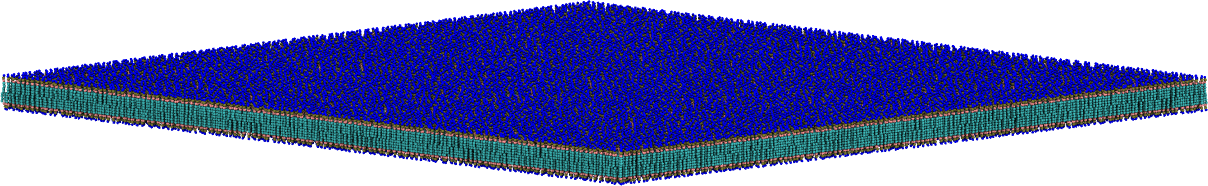
\includegraphics[width=0.4\textwidth]{DPPC_100x100_initial.png}};
    %%     \draw[<->,thick] ([xshift=0.1cm,yshift=0.4cm]a.south west) --node[below,sloped]{\small\SI{100}{nm}} ([xshift=3cm,yshift=.1cm]a.south west);
    %%     \draw[<->,thick] ([xshift=5.75cm,yshift=0.45cm]a.south west) --node[below,sloped]{\small \SI{100}{nm}} ([xshift=3.1cm,yshift=.1cm]a.south west);
    %%     \node at ([yshift=-1.5cm]a){\scriptsize Lipids and solvent: 1.2 Millon beads};
    %%     \node at ([yshift=-2cm]a){\scriptsize $\sim$ 14 million atoms};
    %%   \end{tikzpicture}
    %% };
     

      \node[](a1) at(3.,-0.5){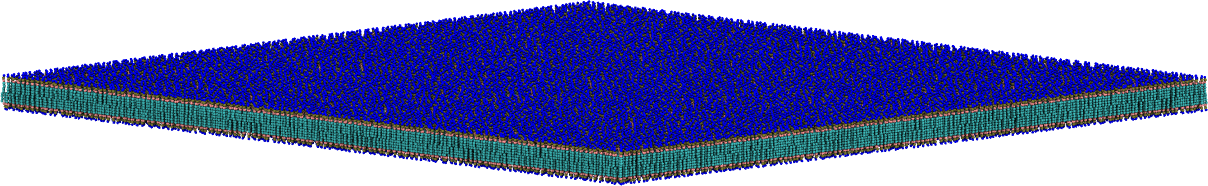
\includegraphics[width=0.65\textwidth]{DPPC_100x100_initial.png}};

      \node[](a2) at(3.,-2.5){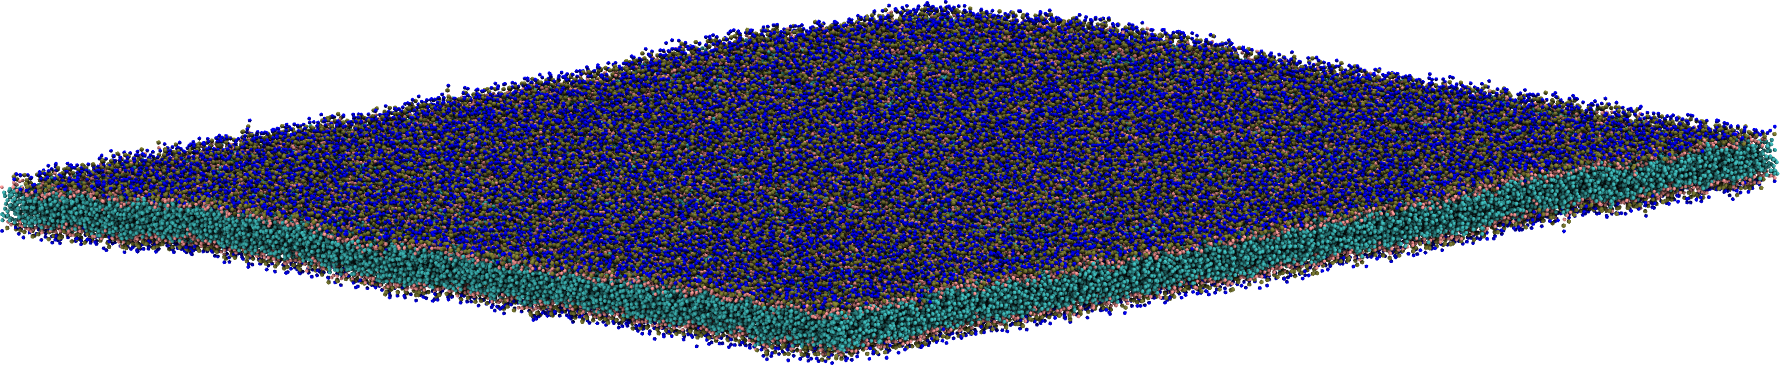
\includegraphics[width=0.65\textwidth]{DPPC_100x100_final.png}};

      \draw[->,ultra thick]([yshift=0.1cm]a1.south)--([yshift=-0.15cm]a2.north);
      \node(b) at(2,-1){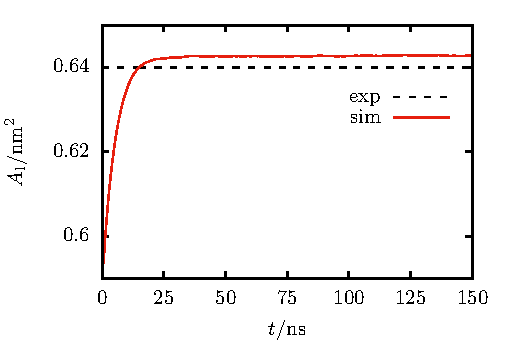
\includegraphics[width=1\textwidth]{dppc_area.pdf}};


      \node(a)at(3,-2){
        \begin{tikzpicture}
        %\node[](a) at(0,0){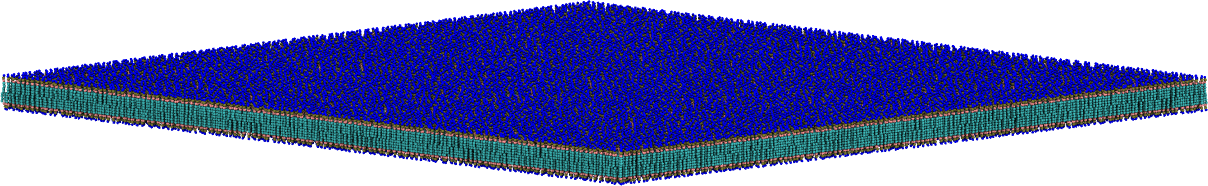
\includegraphics[width=0.65\textwidth]{DPPC_100x100_initial.png}};
        %% \draw[<->,thick] ([xshift=0.1cm,yshift=0.4cm]a.south west) --node[below,sloped]{\SI{100}{nm}} ([xshift=3cm,yshift=.1cm]a.south west);
        %% \draw[<->,thick] ([xshift=5.75cm,yshift=0.45cm]a.south west) --node[below,sloped]{\SI{100}{nm}} ([xshift=3.1cm,yshift=.1cm]a.south west);
        \end{tikzpicture}
      };
      %% \draw[blue,ultra thick] (-1.6,-2.7) circle (0.25cm);

      %% \draw[blue,ultra thick] (7.1,0.1) circle (0.25cm);

  \end{tikzpicture}
\end{document}
